
\renewcommand{\EntradaBibtex}{CruzdeMalta_2017}

\begin{frame}{\citetitle{\EntradaBibtex} \footnotemark[1] (1)}
%\begin{block}{Simulación del Mecanismo de la Cruz de Malta\footnotemark} 
	\begin{itemize}
	\item Se modelaron los componentes individuales 3D (cilindros, tetaedros, etc)
	\item Se incorporó texturas, iluminación y sombras
	\item Es posible ver el modelo desde múltiples perspectivas
	\end{itemize}
\begin{columns}
	\begin{column}{0.48\textwidth}
    \begin{center}
     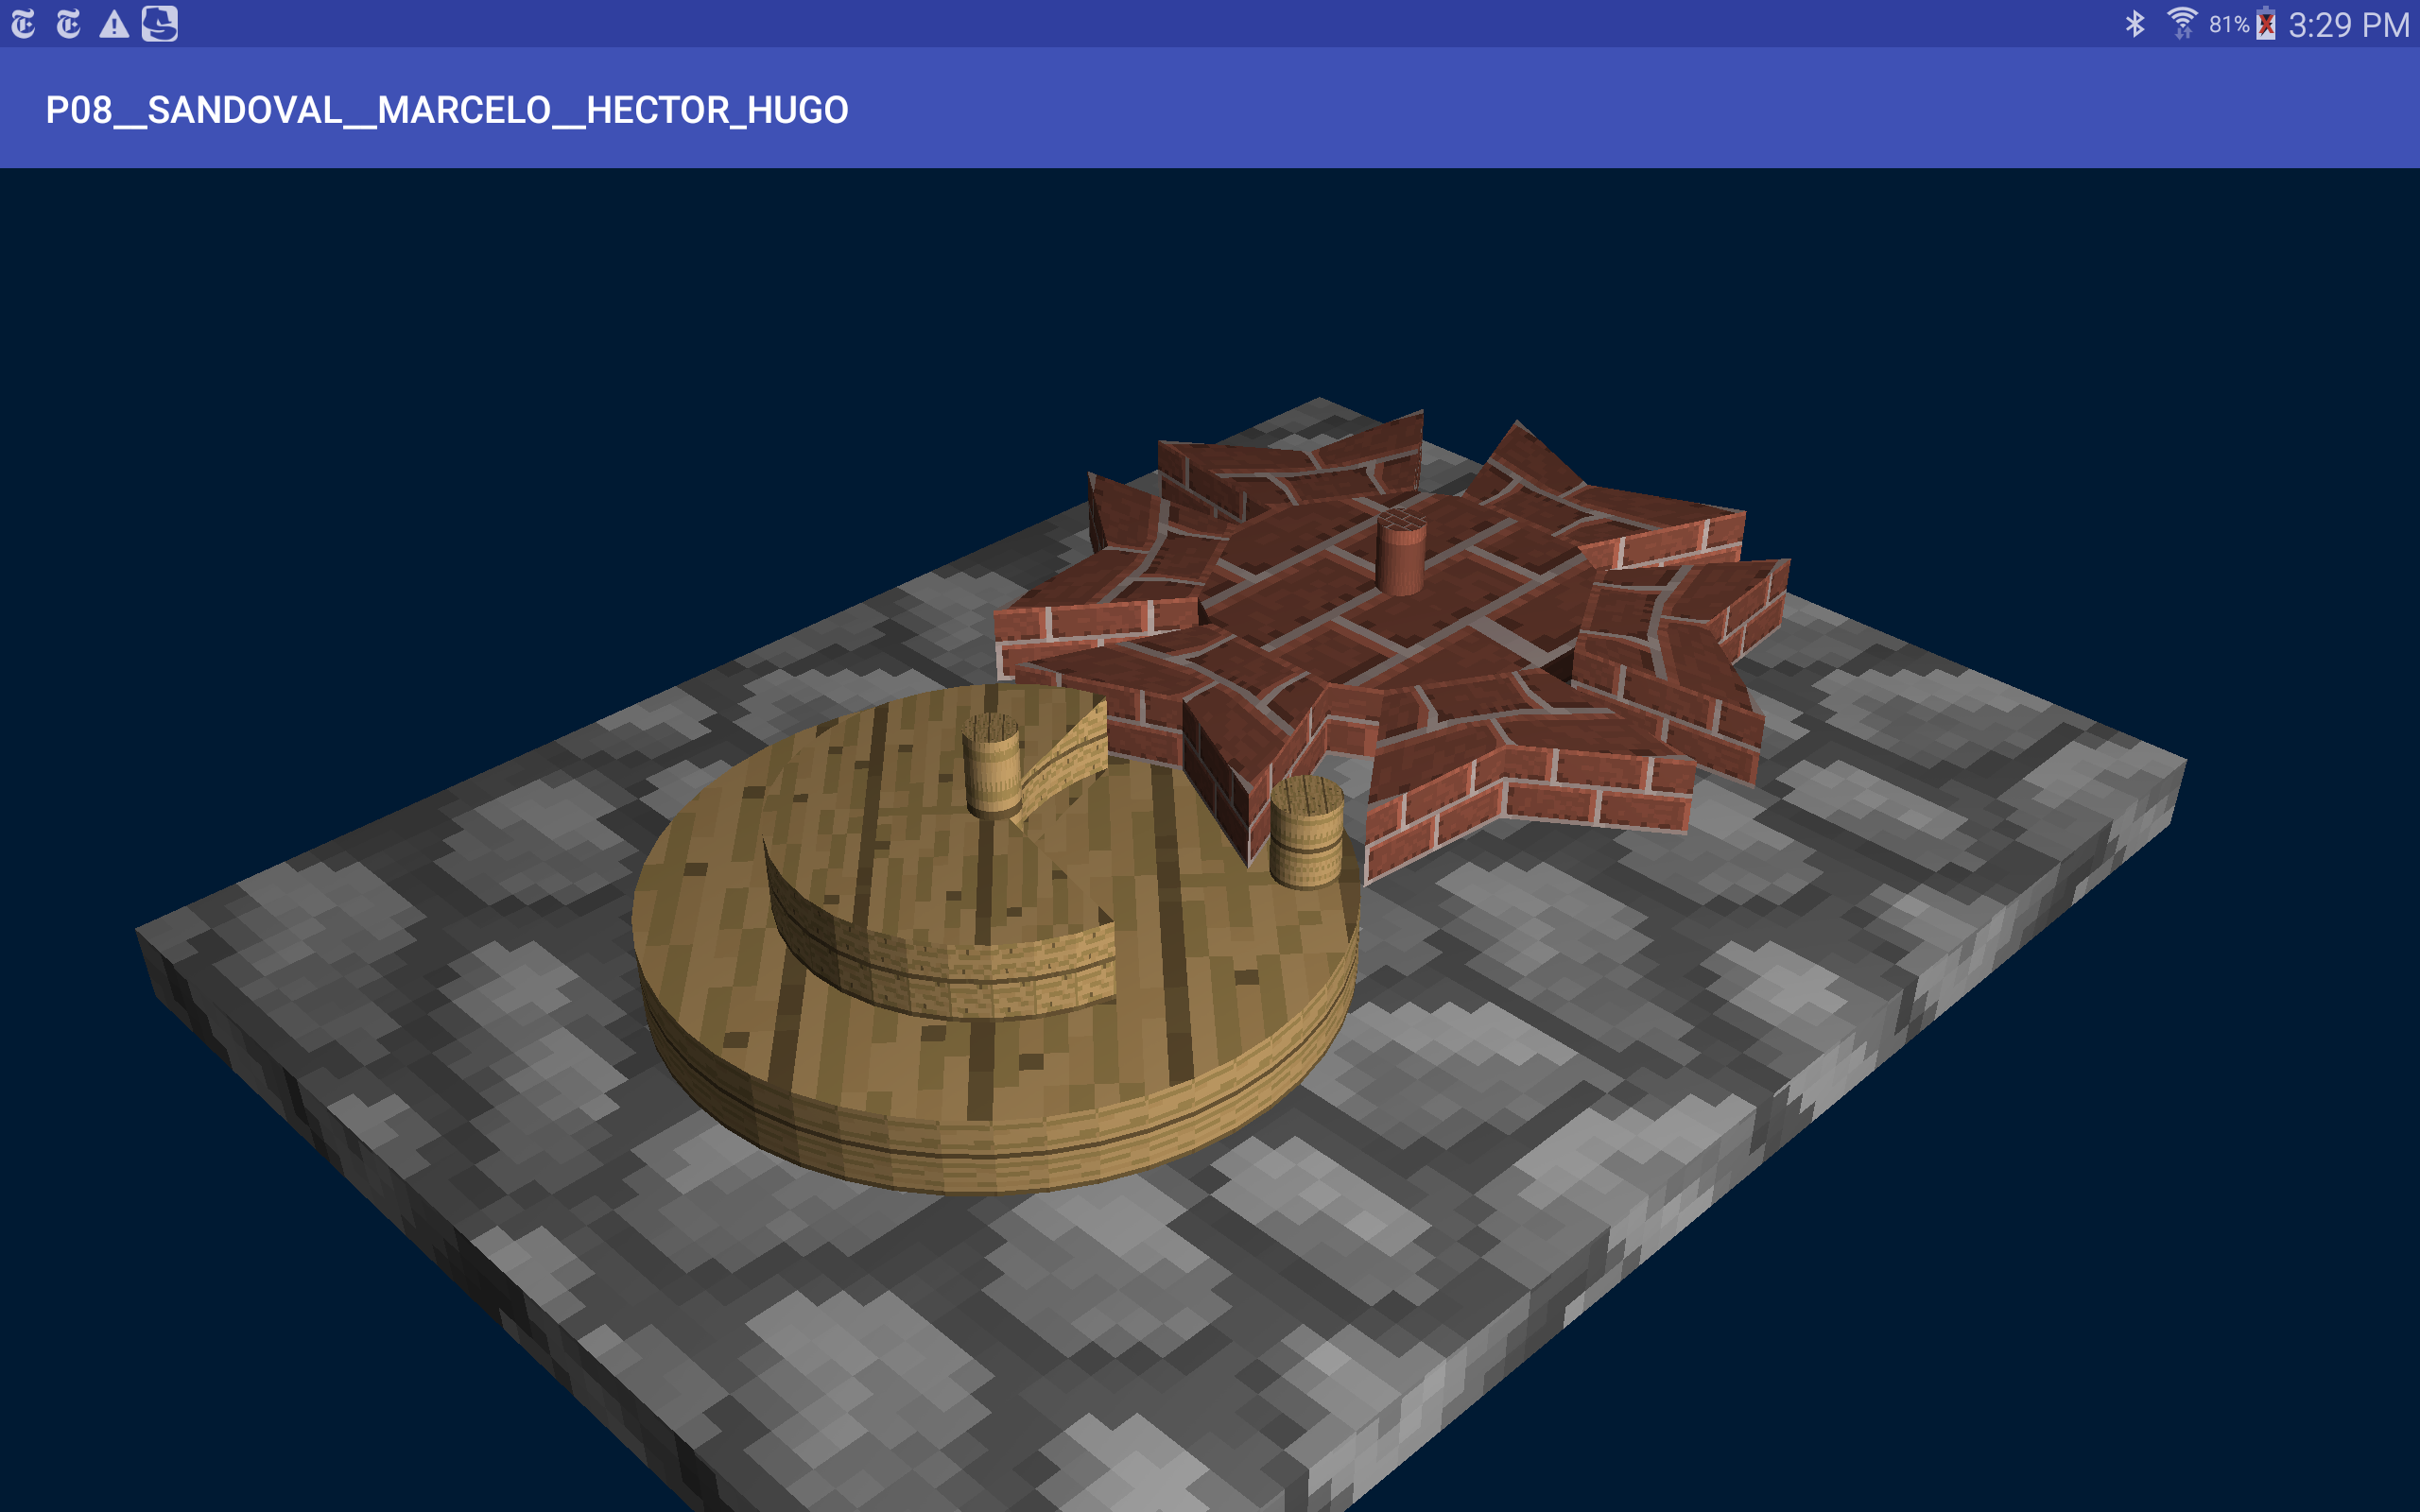
\includegraphics[width=0.7\textwidth]{Figs/CruzMalta_01}
     \end{center}
\end{column}
\begin{column}{0.48\textwidth}  
    \begin{center}
     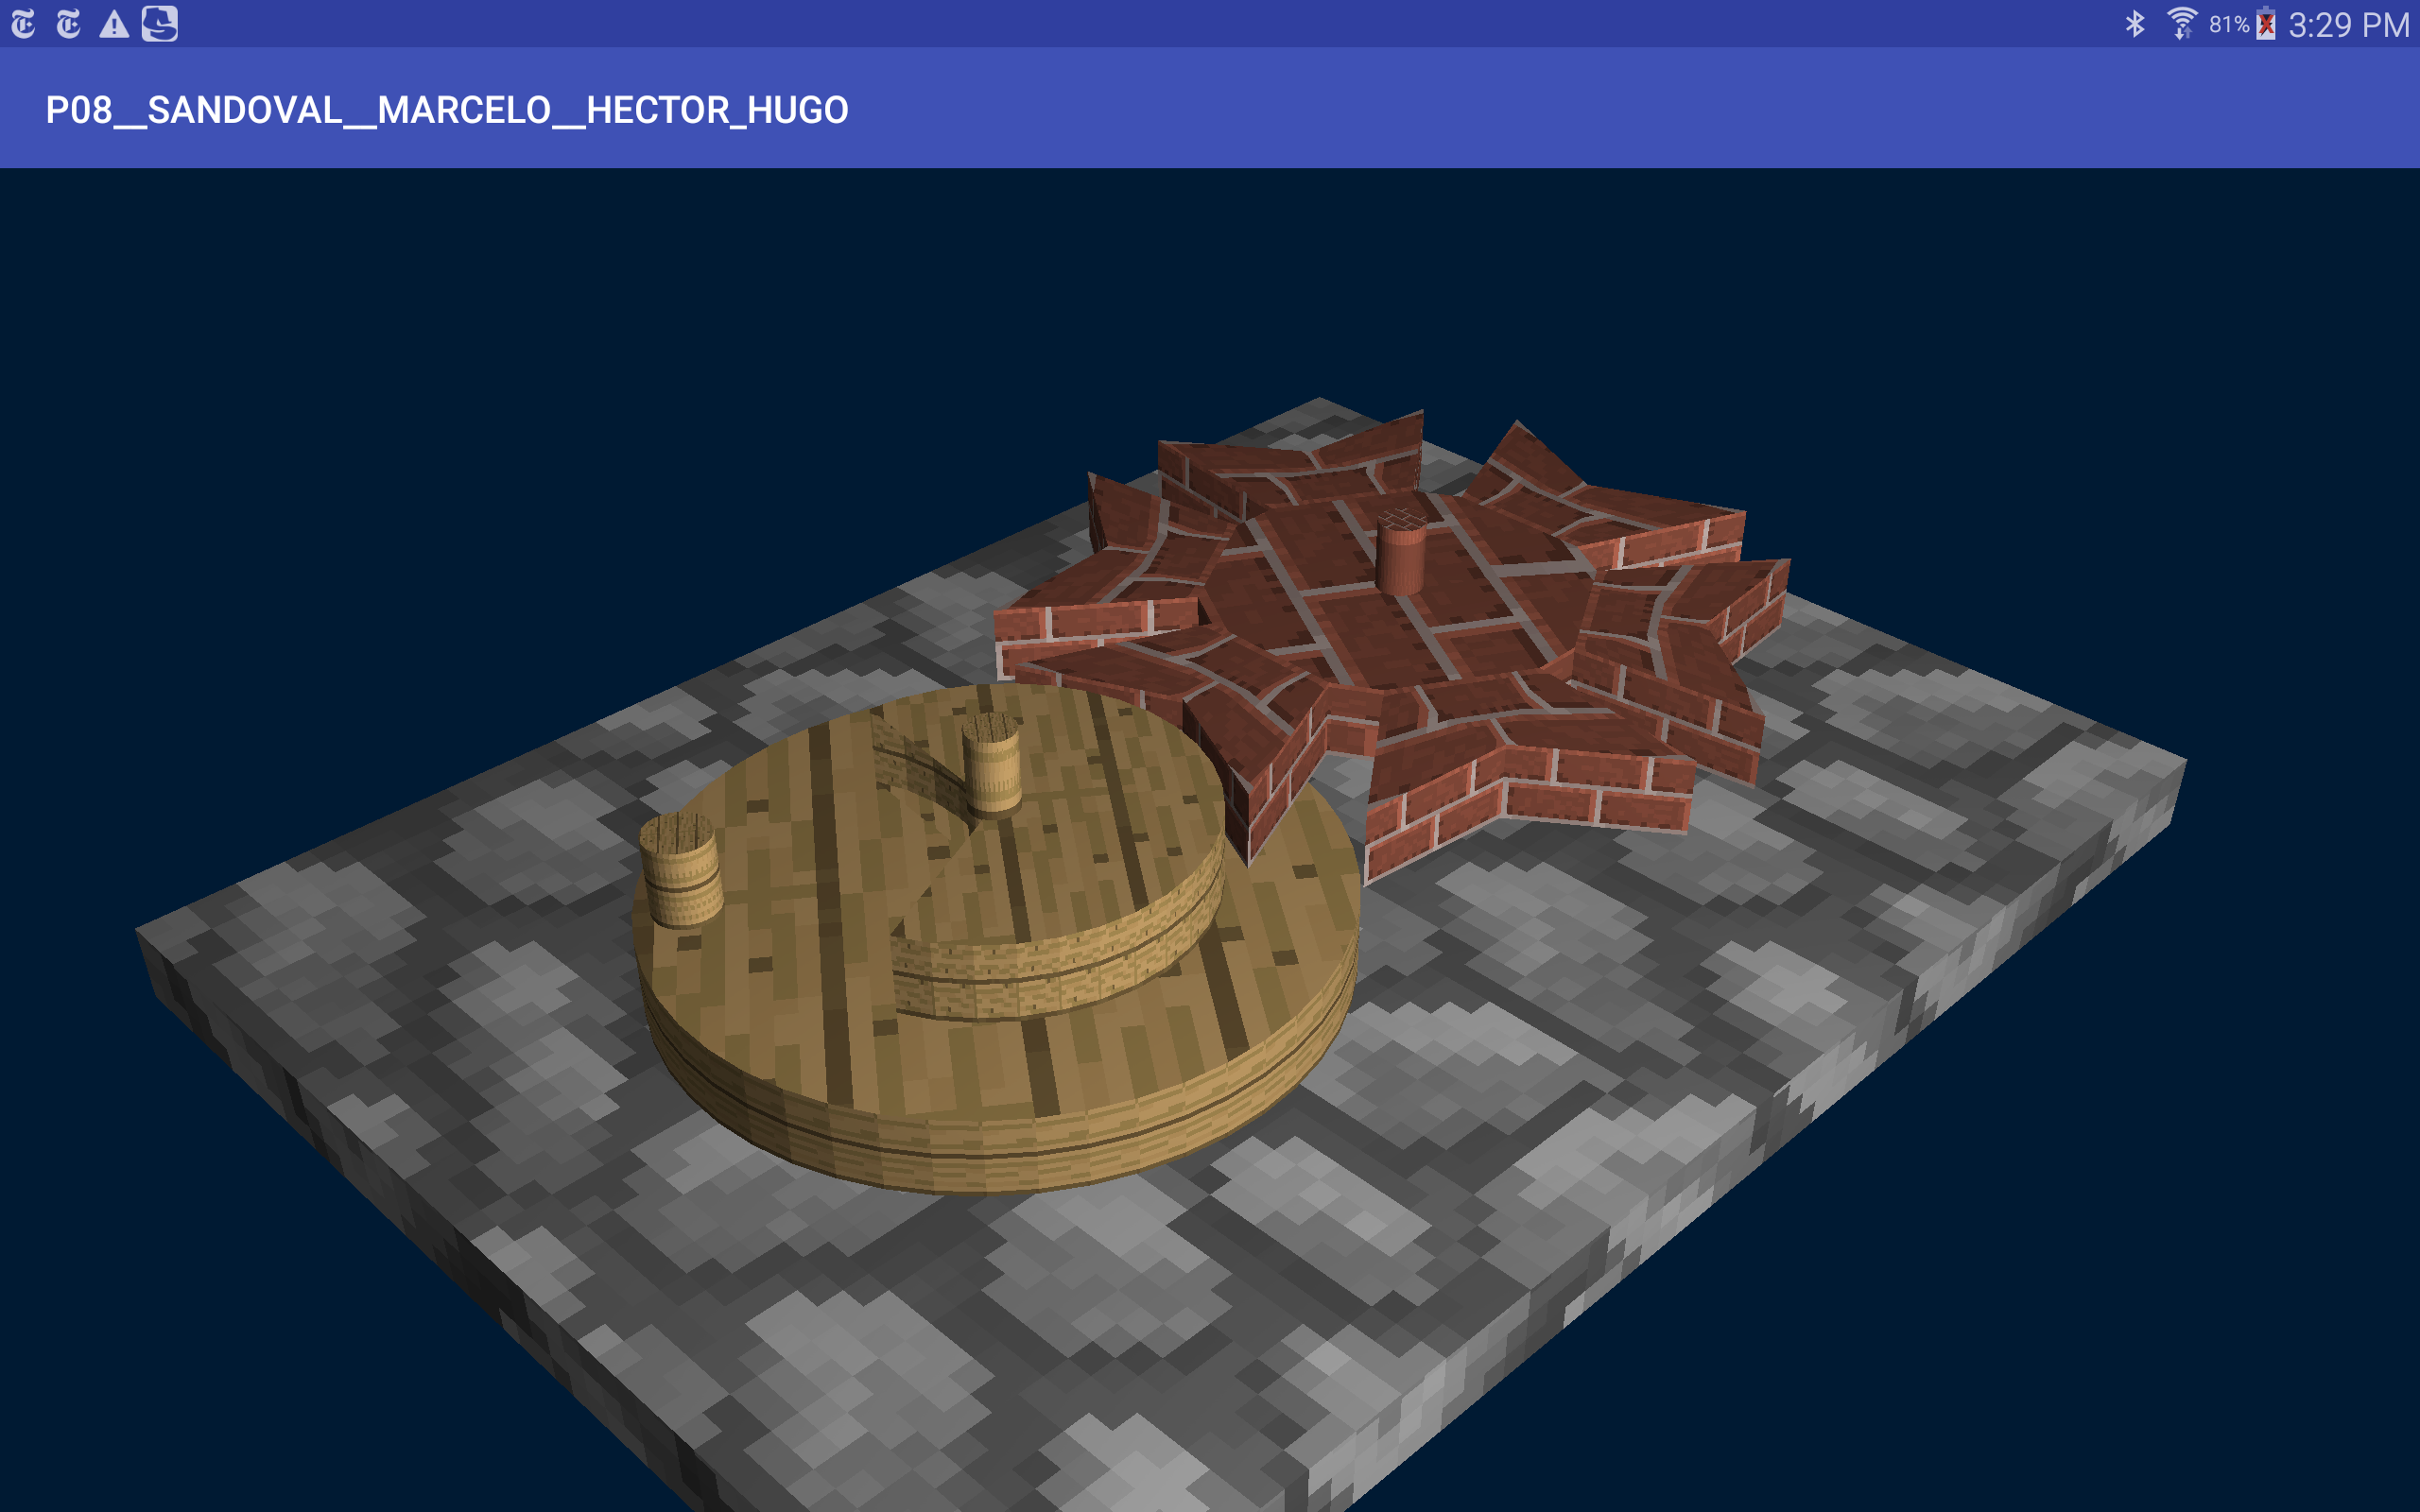
\includegraphics[width=0.7\textwidth]{Figs/CruzMalta_02}
     \end{center}
\end{column}
\end{columns}
%\end{block} 
\footnotetext[1]{\fullcite{\EntradaBibtex}}
%\footnotetext{Héctor Hugo Sandoval Marcelo. \textbf{Movimiento de la Cruz de Malta con Iluminación y Texturas con Java y OpenGL ES 2.0 en Android.}. Universidad Politécnica de Victoria,  Informe técnico proyecto de asignatura ``Graficación por Computadora Avanzada'', 2017. Sin Publicar.}
%\\setcounter{footnote}{0}
\end{frame}


